\documentclass[11pt,a4paper,twocolumn]{article}

\usepackage{amsfonts}
\usepackage{amsmath}
\usepackage[showframe]{geometry}
\usepackage{xcolor,graphicx}
\usepackage[subfolder,cleanup]{gnuplottex}
%\usepackage{amsthm}
%\usepackage{enumitem}
%\usepackage{wrapfig}
\usepackage{subcaption}
%\usepackage{hyperref}
\usepackage{tikz}

\usepackage{lipsum}

\usetikzlibrary{%
	decorations.pathreplacing,%
 	decorations.pathmorphing%
}

%\usepackage[table]{xcolor}
%\rowcolors{2}{gray!25}{white}

\let\originalleft\left
\let\originalright\right
\renewcommand{\left}{\mathopen{}\mathclose\bgroup\originalleft}
\renewcommand{\right}{\aftergroup\egroup\originalright}

\newcommand{\df}{\, \textrm{d}}
\newcommand{\e}{\textrm{e}}
\newcommand{\diff}[3][]{\frac{\df^{#1}#2}{\df{#3}^{#1}}}
\newcommand{\pdiff}[3][]{\frac{\partial^{#1}#2}{\partial{#3}^{#1}}}
\newcommand{\eps}{\varepsilon}
\providecommand{\bigO}[1]{\ensuremath{\mathop{}\mathopen{}\mathcal{O}\mathopen{}\left(#1\right)}}

\definecolor{Beer}{HTML}{FFCC00}

\bibliographystyle{ieeetr}

\title{}
\author{Brady Metherall}
\date{11 November 2019}

\newgeometry{margin=2cm}
%\setlength\parindent{0pt}

\begin{document}
\maketitle

\begin{figure}[tbp]
\centering
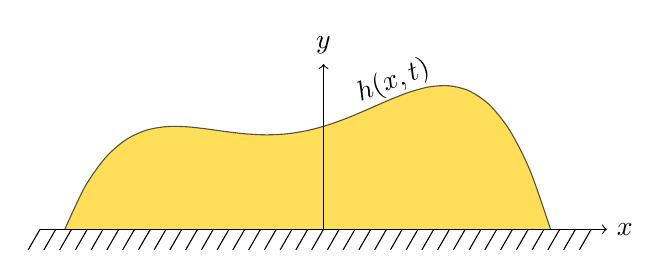
\begin{tikzpicture}[scale=0.6]
% Beer outline
\draw [scale=4,domain=-1.36921:1.20148,smooth,variable=\x,fill=Beer,opacity=0.65] plot ({\x)},{0.5 * (1 - (\x*\x - 1) * (\x + 3/10)^2)});
% Label
\node at (1.6,4*0.7058) [anchor=south,rotate=21.4,yshift=-1mm] {$h(x,t)$};
% Table
\draw [->] (-6,0) -- (6,0) node [right] {$x$};
\draw [decorate,decoration={border,angle=-120,amplitude=3mm,segment length=2mm}] (-6,0) -- (6,0);
% y axis
\draw [->] (0,0) -- (0,3.5) node [above] {$y$};
\end{tikzpicture}
\caption{Beer spilled on a table.}
\label{fig}
\end{figure}

$\eps := H / L \ll 1$

\begin{align*}
\rho \left( \pdiff{\mathbf{u}}{t} + \left( \mathbf{u} \cdot \nabla \right) \mathbf{u} \right) &= - \nabla p + \mu \nabla^2 \mathbf{u} + \rho \mathbf{g}
\end{align*}

\begin{align}
\text{Re}' \left( u_t + u \, u_x + v \, u_y \right) &= - p_x + \eps^2 u_{xx} + u_{yy}, 
\end{align}

\begin{multline}
\text{Re}' \eps^2 \left( v_t + u \, v_x + v \, v_y \right) = \\
- p_y + \eps^4 v_{xx} + \eps^2 v_{yy} - 1
\end{multline}

\begin{align}
\bigO{1}: p_x = u_{yy} \\
\bigO{1}: p_y = -1
\end{align}

\begin{align}
u = -\frac{1}{2} \left( 2hy - y^2 \right) h_x
\end{align}

integrate to find flux

conservation of mas then becomes

\begin{align}
h_t = \frac{1}{3} \nabla \cdot \left( h^3 \nabla h \right)
\label{eq:height}
\end{align}

\begin{align}
\int_\mathbb{R} h \df x
\label{eq:int}
\end{align}

$h(x,t) = t^\alpha f(\eta)$ where $\eta = x t^{-\beta}$

$\alpha = -1/5$ $\beta = 1/5$

\begin{align*}
\frac{-3}{5} \left( \eta f' + f \right) = \left( f^3 f \right)'
\end{align*}


\begin{align*}
f = \left( \frac{9}{10} \right)^{1/3} \left( \eta_*^2 - \eta^2 \right)^{1/3}
\end{align*}

\begin{align*}
\eta_* &= \left( \frac{6075 \Gamma^6 \left( \frac{2}{3} \right) \Gamma^6 \left( \frac{11}{6} \right)}{16 \pi^9} \right)^{1/10} \\
&\approx 0.747412
\end{align*}

\lipsum[1]


\begin{figure}[tbp]
\centering
\begin{gnuplot}[terminal=epslatex, terminaloptions={color size 2.95in,2in lw 3}]
load './Blues.p'

set grid front
set format x '%.1f'
set format y '%.0f'
set format cb '%.1f'
set xr [-1:1.5]

set xl '$x$'
set yl rotate by 0 '$t$'
set cbl '$h(x,t)$'

set view map

set label 1 'I' at -0.75, 2.42 front center
set label 2 'II' at 0.25, 0.42 front center
set label 3 'III' at 1.25, 2.42 front center
set label 4 'IV' at 0.25, 3.42 front center

sp 'Char.dat' u 1:2:3 w image not, \
'Edges.dat' u 7:8:(0) w l dt 3 lc 8 lw 0.5 not, \
'Edges.dat' u 1:2:(0) w l lc 8 not, \
'Edges.dat' u 3:4:(0) w l lc 8 not, \
'Edges.dat' u 5:6:(0) w l lc 8 not, \
'Shock2.dat' u 1:2:(0) w l lc 8 not
\end{gnuplot}
\caption{$\alpha = \pi / 6$}
\label{fig:}
\end{figure}


\lipsum[2]


\begin{figure*}[tbp]
\centering
\begin{subfigure}{0.5\textwidth}
\centering
\begin{gnuplot}[terminal=epslatex, terminaloptions={color size 3.2in,1.75in lw 3}]
set grid
set format x '%.1f'
set format y '%.2f'
set xl '$x t^{-1/5}$'
set yl '$t^{1/5} h(x,t)$'
set ytics 0.25
set xr [-1:1]
set yr [0:1]
set size ratio -1
p 'Cartesian.dat' u 1:2 w l not
\end{gnuplot}
\caption{}
\label{fig:}
\end{subfigure}%
\begin{subfigure}{0.5\textwidth}
\centering
\begin{gnuplot}[terminal=epslatex, terminaloptions={color size 3.2in,1.75in lw 3}]
set grid
set format x '%.1f'
set format y '%.2f'
set xl '$r t^{-1/8}$'
set yl '$t^{1/4} h(r,t)$'
set ytics 0.25
set xr [-1:1]
set yr [0:1]
set size ratio -1
p 'Polar.dat' u 1:2 w l not
\end{gnuplot}
\caption{}
\label{fig:}
\end{subfigure}
\caption{}
\label{fig:}
\end{figure*}



\section{Polar}
solve \eqref{eq:height} and \eqref{eq:int} in polar

$\alpha = -1/4$ $\beta = 1/8$

\begin{align*}
\frac{-3}{8} \left( 2 \eta f + \eta^2 f' \right) = \left( \eta f^3 f' \right)'
\end{align*}

\begin{align*}
f = \left( \frac{9}{16} \right)^{1/3} \left( \eta_*^2 - \eta^2 \right)^{1/3}
\end{align*}

\begin{align*}
\eta_* &= \left( \frac{1024}{243 \pi^3} \right)^{1/8} \\
&\approx 0.779212
\end{align*}

\begin{figure}[tbp]
\centering
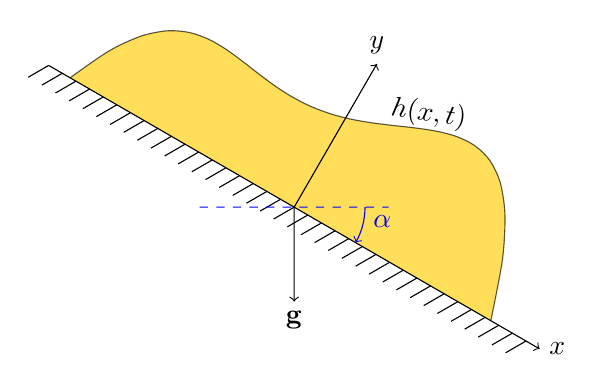
\begin{tikzpicture}[auto,rotate=-30,scale=0.6]
% Beer outline
\draw [scale=4,domain=-1.36921:1.20148,smooth,variable=\x,fill=Beer,opacity=0.65] plot ({\x)},{0.5 * (1 - (\x*\x - 1) * (\x + 3/10)^2)});
% Label
\node at (1.6,4*0.7058) [anchor=south,rotate=21.4-30,yshift=-1mm] {$h(x,t)$};
% Table
\draw [->] (-6,0) -- (6,0) node [right] {$x$};
\draw [decorate,decoration={border,angle=-120,amplitude=3mm,segment length=2mm}] (-6,0) -- (6,0);
% y axis
\draw [->] (0,0) -- (0,3.5) node [above] {$y$};
% Gravity
\draw [->] (0,0) -- (1,-2*0.866) node [below] {$\mathbf{g}$};
% Angle
\draw [dashed,blue] (-2*0.866,-1) -- (2*0.866,1);
\draw [<-,blue] (1.5,0) arc (0:30:1.5) node [pos=0.6,anchor=west] {$\alpha$};
\end{tikzpicture}
\caption{Beer spilled on a crooked table.}
\label{fig}
\end{figure}


\cite{gradshteyn, zwillinger}
\bibliography{Ref}

\end{document}
